% !TEX root = main.tex
\begin{figure}[t]
\centering
	\tikzstyle{block} = [draw, rectangle, minimum height=4em, minimum width=6em]
	\tikzstyle{block1} = [draw, rectangle, minimum height=2em, minimum width=6em]
	\tikzstyle{block2} = [draw, rectangle, minimum height=1em, minimum width=4em]
	\tikzstyle{block3} = [draw, rectangle, minimum height=3.2em, minimum width=4em]
	\tikzstyle{input} = [coordinate]
	\tikzstyle{output} = [coordinate]
	\tikzstyle{pinstyle} = [pin edge={to-,thin,black}]
	{
		
		%\begin{center}
		%\hspace*{\fill} 
		\begin{tikzpicture}[auto,node distance=1cm,>=latex']
		\node [block,text width=3.8cm, pin={[pinstyle]above:$\Delta=\Delta_0$},
		node distance=1cm, align=center, label={[anchor=south east, draw=black, inner sep=1pt]south east:MATLAB}] (RMPC) {Robust explicit MPC\\with disturbance set \Mahmoud{$\mathcal W_{\Delta}$}};
		\Mahmoud{\node [block1,below = 0.8cm of RMPC] (highprec) {High-precision controller (\autoref{eq:affine_map})};}
		%\node[] (partitions) at (2.5,.5){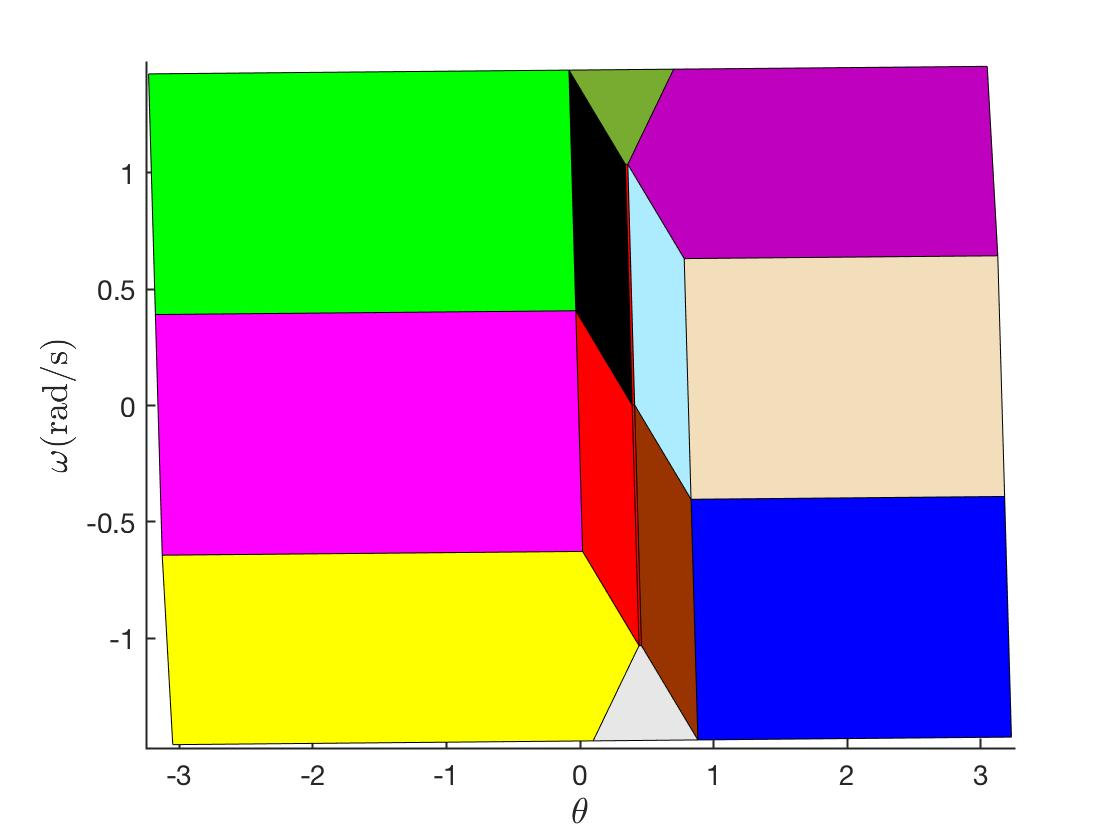
\includegraphics[width=.08\textwidth]{Figs/regs.jpg}};
		\node [block3,below=.8cm of highprec,
		node distance=1cm,text width=4.4cm,  label={[anchor=south east, draw=black, inner sep=1pt]south east:MATLAB}] (Uij) {Incorrect region selection error};
		\node [draw, diamond, minimum height=3em, minimum width=3em, below =0.8cm of Uij, node distance=1cm] (decide) {$e\leq  \Delta$};
		\node [block3, below=0.8cm of decide,node distance=1cm, label={[anchor=south east, draw=black, inner sep=1pt]south east:Daisy}] (done) {Mixed-precision implementation};
		\node [block2, right=1.3cm of decide,
		node distance=1cm] (delta) {\Mahmoud{ $\Delta=e+\varepsilon_{SAFE}$}};
		\node [block1,below = 0.8cm of done] (output) {Low-precision controller \Mahmoud{(\autoref{eq:affine_map})}};
		%\node [scale=1] at (3,-.25)  {$u(x)=Kx+v$};
		\node at (9,-.25) {$e$};
		
		
		\draw [draw,->, align=center] (RMPC) -- node [left] {}(highprec);
		\draw [draw,->, align=center] (highprec) -- node [left] {}(Uij);
		%\draw [draw,->, align=center] (RMPC) -- node [left] {High-precision controller}(Uij);
		\draw [->] (Uij) -- node [left] {$e$}(decide);
		\draw [->] (decide) -- node [left,pos=.3] {Yes} (done);
		\draw [->] (decide) -- node[pos=0.99] {} 
		node [] {No} (delta);
		\draw [->] (delta) |- node [above] {} (RMPC);
		\draw [->] (done) -- node [above] {} (output);
		%\node [block2, scale=0.7] at (1.3,-.42) {MATLAB} ;
		%\node [block2, scale=0.7] at (1.65,-2.95) {Daisy} ;
		%\node [block2, scale=0.7] at (1.58,-7) {Daisy} ;
		\end{tikzpicture}\par}
	%	\hspace{\fill} 
	%\end{center}
	%\end{adjustbox}
	\caption{Overview of the proposed memory-efficient robust EMPC control design.}
	\label{fig:overview}
\end{figure}

\section{Overview}
\label{sec:example}


As a smaller example, consider the standard problem of designing a controller for an inverted pendulum depicted in~\autoref{fig:inverted_pendulum}~{(a)}.
The goal of the controller is to keep the pendulum at the vertical position while satisfying hard constraints on the state variables and control inputs.
A model of the system can be constructed using physical principles. 
After linearization and time discretization, the model is
	\begin{equation}
		\begin{bmatrix}
			 \theta_{k+1}\\
			\omega_{k+1}
		\end{bmatrix}=
		\begin{bmatrix}
			1 & T_s\\
			\frac{T_sg}{L}& (1-\frac{T_sb}{mL^2})		
		\end{bmatrix}
		\begin{bmatrix}
			\theta_k\\
			\omega_k
		\end{bmatrix}+
		\begin{bmatrix}
			0\\
			\frac{T_s}{mL^2}
		\end{bmatrix}u_k + w_k
		\label{eq:pendul_ss}
	\end{equation}
where $\theta_k$, $\omega_k$, and $u_k$ denote respectively the angular position, angular speed, 
and the input torque at time $kT_s$ with $T_s$ being an appropriate sampling time.
The disturbance $w_k\in\mathbb R^2$, bounded with a polyhedral set $w_k\in \mathcal W$, captures the modeling error due to 
linearization and discretization. 
The parameter $g=9.81 [m/s^2]$ is the gravitational acceleration, $m$ is the ball mass, $b$ is the rotational fraction coefficient, 
and $L$ is the length of the bar. 
Starting from an initial state $(\theta_0,\omega_0)$, the control goal is to converge to the equilibrium point 
$\theta=0, \omega=0$.
Additionally, we require the state constraints $\theta_k\in[-\pi,\pi]$ and $\omega_k\in[-\pi/8,\pi/8]$ to hold at all time instances.

%\begin{figure}[t]
%	\centering
%  \begin{subfigure}[b]{0.33\columnwidth}
%      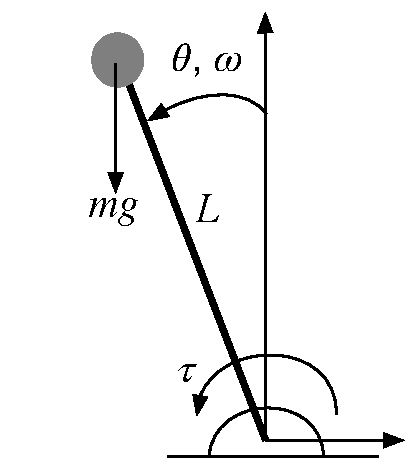
\includegraphics[width=\textwidth]{Figs/inverted_pendulum.pdf}
%      \vspace{0.05cm}
%      \caption{}
%  \end{subfigure}
%  %~ %add desired spacing between images, e. g. ~, \quad, \qquad, \hfill etc. 
%  \begin{subfigure}[b]{0.66\columnwidth}
%      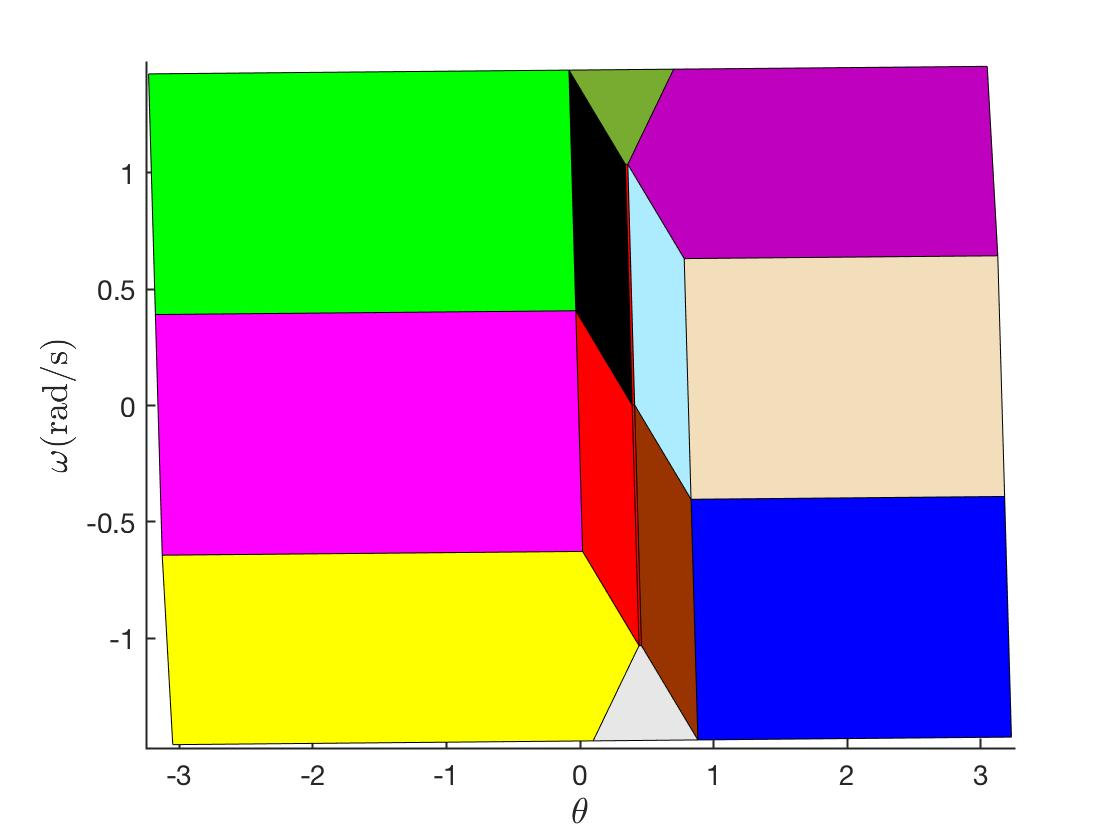
\includegraphics[width=\textwidth]{Figs/regs.jpg}
%      \caption{}
%  \end{subfigure}
%	\caption{(a) Inverted pendulum; (b) 2D plot of polyhedral partitions for an EMPC applied to the inverted pendulum.}
%	\label{fig:inverted_pendulum}
%\end{figure}

Our overall goal is to 
(i) design a robust MPC controller that achieves the performance objectives including hard constraints in spite of an additional bounded
disturbance $\Delta$ modeling the implementation error (both errors due to choosing a wrong region and the finite-precision computation of the control action);
and at the same time
%\eva{what about the modelling error that $\Delta$ bounded in the paragraph before?}
(ii) to minimize the total number of bits that are required to represent an explicit controller.

% There are many control schemes that can guarantee convergence of the trajectories to the rest position (e.g., state feedback or linear quadratic regulator), but fail to ensure hard constraints on the states at all time instances. The main feature of MPC schemes is to automatically include these constraints in the design of control actions.
%	One major challenge of implementing model predictive controllers over embedded systems is to solve the related optimization within each sampled time inerval. Since the system under consideration is LTI, one can use explicit MPC \cite{Bemporad:2002} that computes partitions over state space together with affine functions which are then used to compute the optimal control input over their corresponding partition. For the inverted-pendulum example, the computed controller contains $12$ partition presented in Fig.~\ref{fig:inverted_pendulum}~{(b)}, each with an affine function that gives the control action over that partition.
	
%	In many practical applications, explicit MPC is implemented over relatively low-price embedded systems with limited memory capacity and computational power. The partitions together with the affine functions should be stored on the embedded system.
%	Computing the control action, i.e., evaluating the affine function for a specific state, can be performed efficiently using for example binary tree search. However, the memory limitations is more crucial since the memory usage increases linearly with the number of partitions.
%	In this paper we discuss a method for reducing the memory usage in applying explicit MPC to LTI dynamical systems.
	
%	Many low-end embedded systems only support fixed point arithmetic which causes errors that is inversely proportional to the number of bits used for representing each variable. It is necessary to account for such errors in the design stage of the controllers to be able to enforce hard constraints on the states at the final implementation of the controller. Our proposed method iteratively solves a robust version of the MPC with varying bound on the disturbance to include such errors.   %Therefore, one needs to formulate the problem as robust EMPC to count for disturbance input $|\delta|\leq \Delta$ which is summed up with the control input torque $u$ in each time step.
	 %Setting the number of bits for storing different variables, one can compute the upper bound for approximation error, $\bar\omega$.
	%However, we would like to achieve the minimum number of bits to reduce memory requirements.
	
%	In summary, we design a robust explicit MPC, taking fixed-point arithmetic errors into account and find a minimal set of mixed precision assignments for all the quantities that must be stored on the embedded system. 
% Denote the overall error produced by the fixed finite precision implementation by $e$.

%Our approach iteratively expand the bound on disturbance $\Delta+\Delta_0$, designs a robust explicit MPC controller with this bound and 
% uses state-of-the-art fixed-point error analyzers to find the minimum total number of bits for storing the controller into the embedded system with maximum error $\Delta_0$.
	
Figure \ref{fig:overview} gives a high-level overview of our proposed setup.
We start by selecting an initial bound $\Delta_0$ on the implementation error and enlarge $\mathcal W$ with $\Delta_0$ as $\mathcal W_{\Delta_0}$, where
\begin{equation}\label{eq:W_delta}
\mathcal W_{\Delta} := \{w_1+w_2 \,|\, w_1\in \mathcal W, \|w_2\|\le \Delta\}
\quad\text{ for all } \Delta\ge 0.
\end{equation}
 
For our example, we choose $\Delta_0=0.01$ and $\mathcal W = \{0\}$. 
We use Matlab to find a robust explicit MPC with disturbance set $\mathcal W_{\Delta_0}$. 
%
The output of robust EMPC given by Matlab decomposes the control domain into a
finite number of polyhedral domains together with an affine map for each domain. 
At each time step, the state vector $x_k$ is read (or estimated) and based on the domain
that it belongs to, the corresponding control output is computed. 
However, the polyhedral regions are implemented in finite precision so that
it is possible that due to quantization errors the domain is selected incorrectly, and therefore
a different affine map is computed for the control.
We refer to the resulting error as \emph{incorrect region selection} error.
% However, due to error by fixed-point implementation, it is possible that the domain is selected
% incorrectly. This causes an error term which we refer to it as incorrect region
% selection error.
In our example, we compute an incorrect region selection error $e = 0.019$, which is larger
than $\Delta_0=0.01$. We therefore increase the disturbance bound by a fixed amount \Mahmoud{$\varepsilon_{SAFE}=0.031$} to
$\Delta_1 = 0.05$ and enlarge the disturbance set as $\mathcal W_{\Delta_1}$. 

%
Solving the robust explicit MPC problem for this enlarged disturbance set gives the new controller
with 14 regions, shown in~\autoref{fig:inverted_pendulum}(b).
A sample region with the corresponding affine map is shown below:
\begin{equation*}
\resizebox{.9\hsize}{!}{$
\begin{bmatrix}
-0.005  &0.999\\
-0.998  &-0.049\\
0.005  &-0.999\\
0.998   &0.049
\end{bmatrix}x_k\leq 
\begin{bmatrix}
0.416\\
3.157\\
0.617\\
-0.0124
\end{bmatrix}
\Rightarrow
u(x_k)=\begin{bmatrix}
0.05&-9.67
\end{bmatrix}x_k+4.02$}
\end{equation*}
where the output of robust EMPC at state $x_k$ is denoted by $u(x_k)$. 
The remaining mappings have a similar structure.
For this new controller, the incorrect region selection error is 
approximately $e = 0.019$, which is now below the disturbance bound $\Delta_1$,
so that we can continue with the precision assignment.

%\begin{equation}
%\kappa(x_k)=
%\begin{cases}
%.05x_k-9.67 & \text{if $x_k\in \mathcal{R}_1$}\\
%F_2x_k+G_2 & \text{if $x_k\in \mathcal{R}_2$}\\
%\vdots\\
%F_Px_k+G_P & \text{if $x_k\in \mathcal{R}_P$}
%\end{cases} 
%\end{equation}

Next, we use the precision tuning tool Daisy \cite{Daisy} to provide a mixed-precision 
implementation for all the parameters which satisfies the error bound $\Delta_1  - e = 0.05 - 0.019 = 0.031$.
The mixed-precision implementation returned by Daisy requires $6084$ bits.
Thus, \Mahmoud{for this introductory example,} the mixed-precision implementation takes about $10\%$ less memory compared 
to the smallest uniform precision implementation that respects $\Delta_1$,
and about $57\%$ less memory than an implementation that uniformly uses
32 bits.

	
	
%	\tikzstyle{block} = [draw, rectangle, 
%	minimum height=3em, minimum width=6em]
%	\tikzstyle{sum} = [draw,  circle, node distance=1cm]
%	\tikzstyle{input} = [coordinate]
%	\tikzstyle{output} = [coordinate]
%	\tikzstyle{pinstyle} = [pin edge={to-,thin,black}]
%	\begin{figure*}[t]
%		\begin{tikzpicture}[auto, node distance=2cm,>=latex',scale=1]
%			\centering
%			\node [block,scale=1,,text width=3.5cm, pin={[pinstyle]above:$\Delta=\Delta_0$},
%			node distance=1cm] (RMPC) {Robust explicit MPC design (computed by MATLAB)};
%			%\node[] (partitions) at (2.5,.5){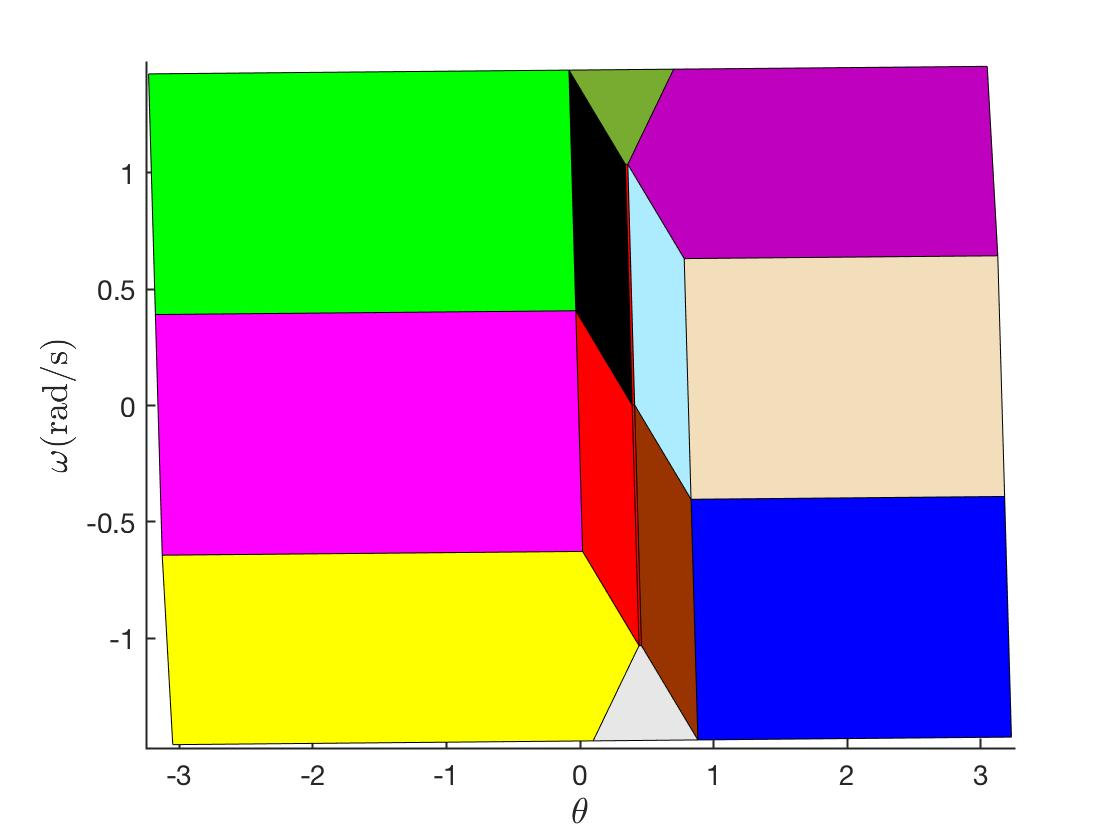
\includegraphics[width=.08\textwidth]{Figs/regs.jpg}};
%			\node [block, scale=1,right=2.5cm of RMPC,
%			node distance=5cm,text width=4cm] (mixed) {Finite precision implementation (computed by Daisy)};
%			\node [draw, diamond, 
%			minimum height=3em, minimum width=3em, right =1cm of mixed,
%			node distance=5cm] (decide) {$e\leq \bar \Delta$};
%			\node [block, right of=decide,
%			node distance=3cm] (done) {Done};
%			\node [block, below of= decide,
%			node distance=3cm] (delta) {increase $\Delta$};
%			\node [scale=1] at (3,-.25)  {
%				$u(x)=Kx+v$
%			};
%		\node at (9,-.25) {$e$};
%			
%			
%			\draw [draw,->] (RMPC) -- node [pos=-.1] {}(mixed);
%			\draw [->] (mixed) -- node [name=aaa] {}(decide);
%			\draw [->] (decide) -- node [above,pos=.3] {Yes} (done);
%			\draw [->] (decide) -- node[pos=0.99] {} 
%			node [] {No} (delta);
%			\draw [->] (delta) -| node [above] {} (RMPC);
%	
%	\end{tikzpicture}
%	\caption{high-level description of the proposed memory-efficient robust MPC design
%\RM{what is $\bar{\Delta}$}
%\RM{try to draw a better picture spanning only one column. the information in this pic is sparse}
%\RM{why is $u$ a single affine map?}
%\RM{why is Daisy only giving $e$? Shouldn't it also return the best mixed precision impl?}
%}
%	\label{fig:overview}
%\end{figure*}
